\chapter{Optimizing Photovoltaic Systems}\label{chapter:optimizing_pv_systems}

In this final chapter, \textbf{Optimizing Photovoltaic Systems}, we explore the
surrounding infrastructure around the solar array that enables it to operate at
its full potential. In particular, we take a look at the \acf{MPPT} \acf{HW}
used to control the solar array and propose a suite of MPPT algorithms that can
address nonidealities in the \ac{I-V} curve that were observed in
\autoref{sec:modeling_solar_arrays} such as global and local \acfp{MPP} and partial
shading effects. We present a comprehensive \ac{PV} system simulator that
incorporates the models discussed in \autoref{chapter:modeling_pvs} and the
high level design developed in \autoref{chapter:optimizing_pvs} to evaluate the
effects of these \ac{MPPT} algorithms in terms of stability, convergence speed,
total efficiency, and so forth. Finally, we implement a set of performant
algorithms in real \ac{HW} and validate that the optimizations and models
perform as expected.


\begin{figure}[h]
    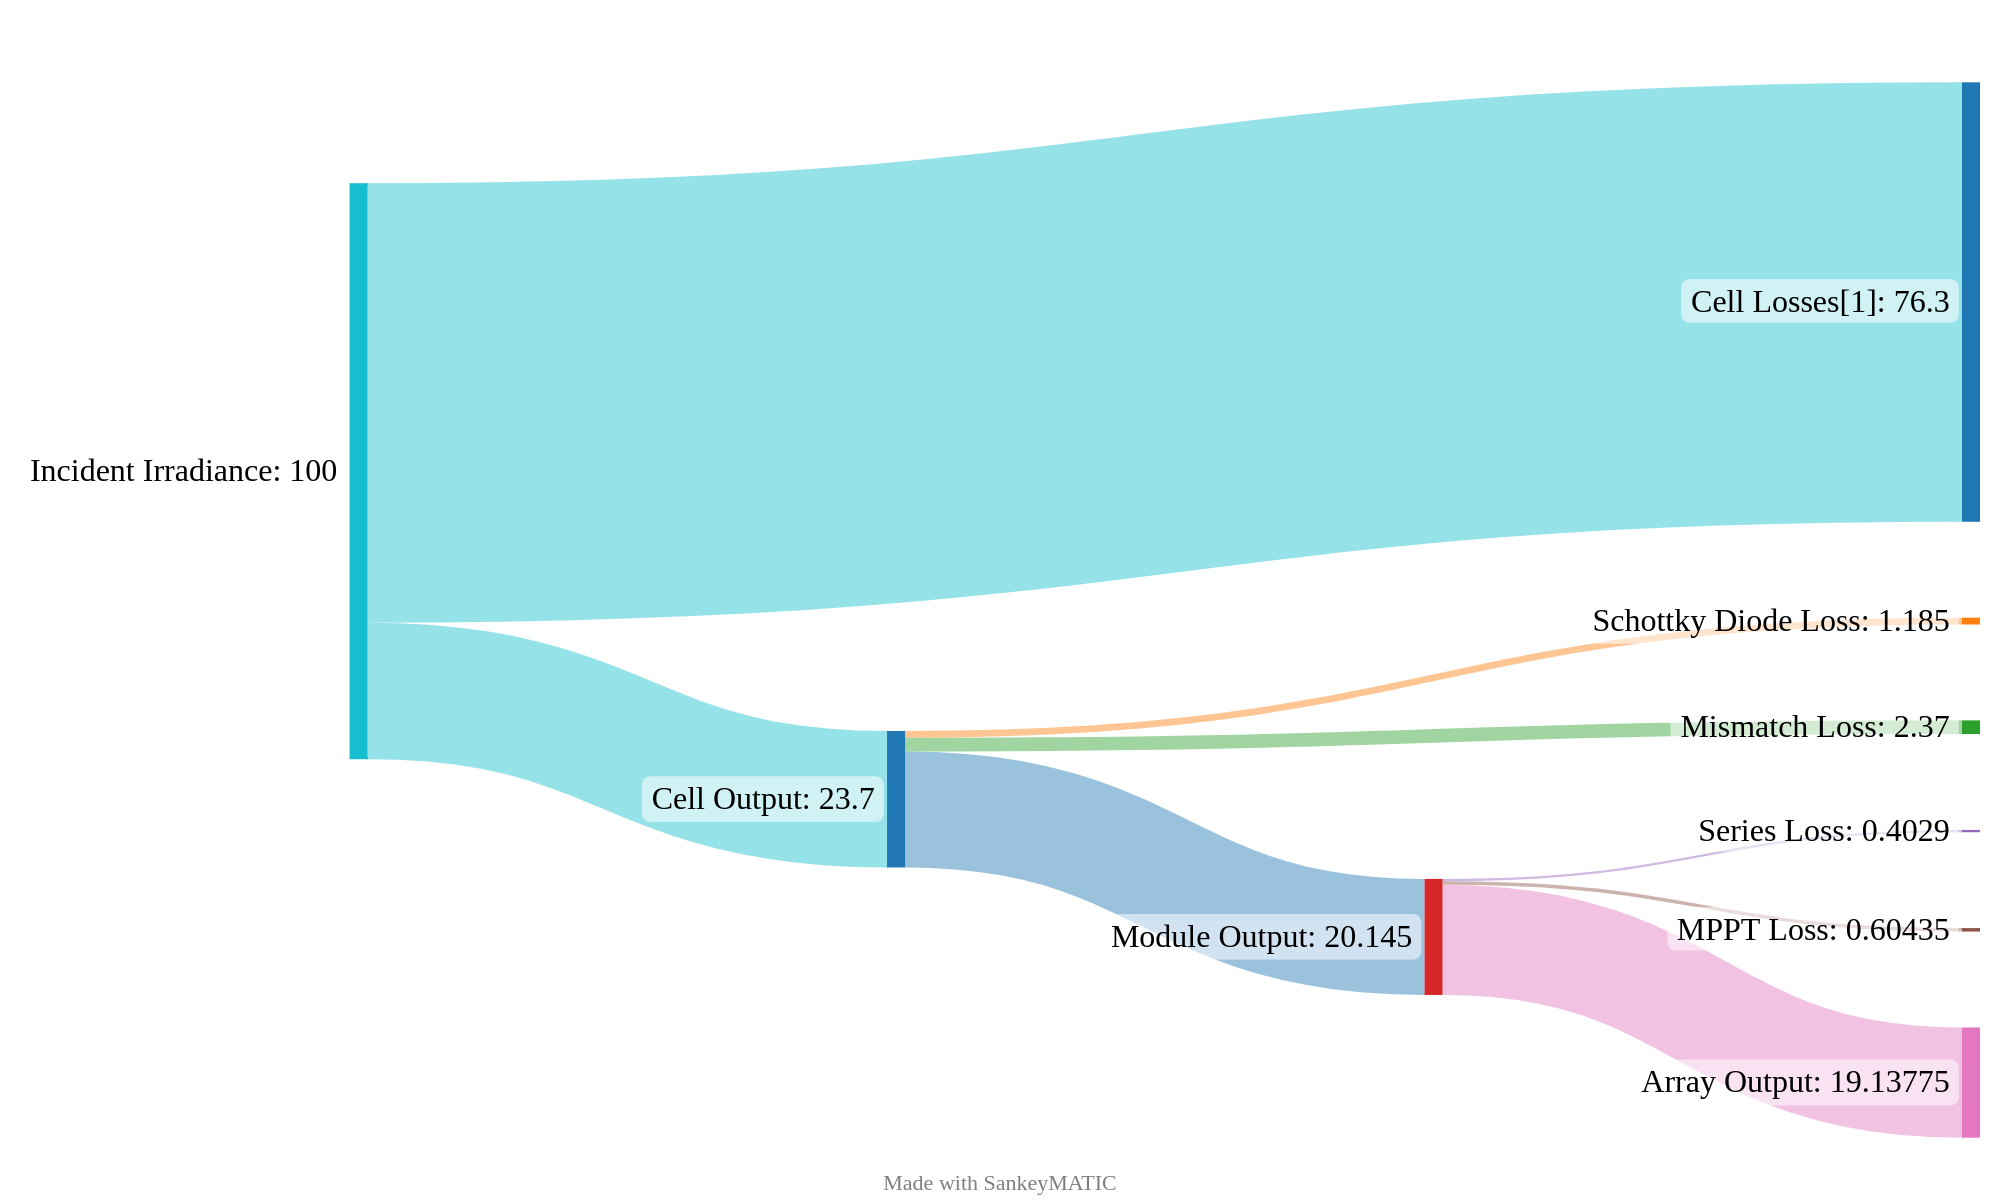
\includegraphics[width=\textwidth]{photovoltaic_system_sankey.png}
    \caption{Sankey Diagram for Photovoltaic System}
    \label{fig:photovoltaic_system_sankey}
\end{figure}

\todo[inline]{Reset sankey with real data}


\section{Conclusion}\label{sec:optimizing_pv_systems_conclusion}

%TODO: conclusion for Chapter 3
\todo[inline]{Insert conclusion on chapter topics and results.}

